
\documentclass[reprint,amsmath,aps,nofootinbib,english]{revtex4-2}

\usepackage{graphicx}
\usepackage{dcolumn}
\usepackage{url}
\usepackage{siunitx}
\usepackage{float}

\AtBeginDocument{\renewcommand{\natexlab}[1]{#1}}% <--- the fix
\begin{document}

\title{Poisson Statistics}
\author{Tan Aytekin}
\email[]{tan.aytekin@boun.edu.tr}
\affiliation{Physics Department, Bogazici University, Istanbul, Turkey}
\collaboration{Partner : Özgür Aydın}
\date{\today}


\begin{abstract}
In this experiment, we tried to study which distribution method is more appropriate to present the phenomenon called radioactive decay. We use gamma-ray source and measured the number of decays in 1 and 10 seconds intervals. After we binned these distributions, we applied poisson and gaussian fits. Using chi-square test, we conclude that poisson fit is more appropirate than gaussian fit for radioactive decay.
\end{abstract}

\maketitle

\section{Introduction}

\subsection{History}
The Poisson distribution was developed by French mathematician Simeon Denis Poisson. He originally develop the poisson distribution in order to find the number of times a gambler would win a rarely won game of chance in a large number of tries.\cite{bri} Later, British statistican R. D. Clarke used poisson distribution to analyze the distribution of hits of flying bombs in London during World War II.\cite{clarke_1946}


\subsection{Theory}
Let $p$ is the probability of success on a single trial. The probability of observing $n$ successes in $N$ independent trials can be easily calculated with binonimal expension:
\begin{align}
        P(n;N,p) &= \binom{N}{n} p^{n} (1-p)^{N-n} \\
                 &= \frac{N!}{n!(N-n)!} p^{n} (1-p)^{N-n}
\end{align}
This is called Binonimal Distribution and it is useful for calculating probability of success in indepently repeated processes like tossing coins, etc.\\

Now consider our number of trials $N$ is too high and probability of success $p$ and number $n$ of interest is too low like our experiment since number of atoms is too much in comparison to number of observed decays.\footnote{1 mole atom approximately equals to $6.02\times 10^{23}$ atoms and our observed decay per second is $\approx 10$ which indicates our possibility is low but not negligible since number of trials is high.} Since $n \ll N$ , we can approximate \cite{berk}:
\begin{align}
        \frac{N!}{(N-n)!} \approx N^n \label{eq:N}
\end{align}
Let y will be the other therm:
\begin{align}
        y &\equiv (1-p)^{N-n} \\
        ln(y) &= (N-n) ln(1-p)
\end{align}
Since $n \ll N$ and $p \ll 1$, we can put $N-n \approx N$ and taylor expand $ln(1-p) \approx -p$.
\begin{align}
        ln(y) \approx -Np \\
        y \approx e^{-Np} \label{eq:y}
\end{align}
Using \eqref{eq:N} and \eqref{eq:y}:
\begin{align}
        P = \frac{N^n}{n!}p^n e^{-Np}
\end{align}
Let mean: $\mu \equiv Np$ we obtain:
\begin{align}
        P = \frac{\mu ^n}{n!} e^{-\mu} \label{eq:poiss}
\end{align}
which is called poisson distribution and it has an interesting property that the standart deviation $\sigma$ is equal to the square root of its mean $\mu$:
\begin{align}
        \sigma^2 = \mu
\end{align}
\\

Now let's look at the case that if the mean value $\mu$ is too large.\cite{gauss}: \\
Let $x$:
\begin{align}
        x &= n = \mu (1+ \delta) \\
        \Rightarrow \delta &= \frac{x - \mu}{\mu} \label{eq:lambda}
\end{align}
where $\mu \gg 1$ and  $ \delta \ll 1$. We can use Stirling approximation when $ x \rightarrow \infty $ :
\begin{align}
        x \approx \sqrt{2 \pi x} e^{-x} x^x
\end{align}
We get:
\begin{align}
        P &= \frac{\mu^{\mu(1+\delta)}e^{-\mu}}{\sqrt {2\pi}  e^{-\mu(1+ \delta)} (\mu(1+\delta))^{ \mu (1+\delta) + 1/2} } \\
          &= \frac{e^{\mu \delta} ( 1 + \delta ) ^ { -\mu (1 + \delta ) +  1/2 }}{ \sqrt{2\pi \mu}}
\end{align}
Taking log and taylor expand to second order $ (1 + \delta ) ^ { -\mu (1 + \delta ) +  1/2 } $ we obtain:
\begin{align}
        P = \frac{e^{\mu \delta^2 /2}}{\sqrt{2 \pi \mu}}
\end{align}
Finally using \eqref{eq:lambda}, we get:
\begin{align}
        P = \frac{e^{- (x-\mu)^2 / 2\mu}}   { \sqrt{2 \pi \mu}} = \frac{e^{- (x-\mu)^2 / 2\sigma ^2}}   { \sigma \sqrt{2 \pi}}
\end{align}
which is called Gaussian Distribution. \\

Now let's try to find the probability of observing n counts during a time interval t \cite{Gulmez}. Let $\mu = \alpha t$ and putting into \eqref{eq:poiss} we get:
\begin{align}
P(\alpha, t, n) = \frac{(\alpha t)^n e^{-\alpha t}}{n!}
\end{align}
The probability of having one success in a time interval dt can be shown:
\begin{align}
P(\alpha, dt, 1) = \frac{(\alpha dt) e^{-\alpha dt}}{1}
\end{align}
The probability of having n successes in a time interval t followed by another success within a dt time is:
\begin{align}
        P(n+1, t) dt &= P(\alpha, t , n) P(\alpha, dt, 1) \\ 
                     &= \frac{(\alpha t)^n e^{-\alpha t}}{n!} \frac{(\alpha dt) e^{-\alpha dt}}{1} 
\end{align}
Since $e^{\alpha dt} \approx 1$ we get:
\begin{align}
        P(n+1,t) = \frac{(\alpha t)^n e^{-\alpha t} \alpha}{n!} \label{eq:time}
\end{align}
Observe that when n gets bigger the distrubition approaches the Gaussian distribution. Thus, n will be limited to 0 and 1 in the experiment.







\section{Experiment}
\subsection{Apparatus}
\begin{itemize}
        \item Sample Holder
        \item Lead Absorber 
        \item Analog Chart Recorder
        \item High-voltage (about 400V) Power Supply 
        \item Gamma-ray Source
        \item Ruler
        \item Geiger Counter
\end{itemize}
\subsection{Procedure}
\subsubsection{First Part}
First in order to determine the operating voltage of the Geiger tube, the source placed onto the sample holder beneath the geiger tube. The counter is set to 100 s and data is taken at 20 V intervals of high-voltage. Then, the number of counts and applied voltages are plotted. The point which the counts reach the approximately constant value is selected. (In our case the voltage is 400V). Later, the counter set to continous mode with 10s interval and about 100 number of counts were recorded. Then, this process repeated with 1s intervals.  
\subsubsection{Second Part}
In this part, in order to find distribution of successive counts, tray position is selected that result in a count rate of 1 per second. Then, time intervals between adjacent pulses are recorded with the analog chart recorder in cm. Later, these values are measured with the ruler.  
\section{Data Analysis}
\subsubsection{First Part}
In this part, first we binned our readings in 10s and 1s intervals to 10 equal width bins. Then, each histogram is normalized. Later, gaussian and poisson fit are applied to each histogram.
\begin{figure}[H]
  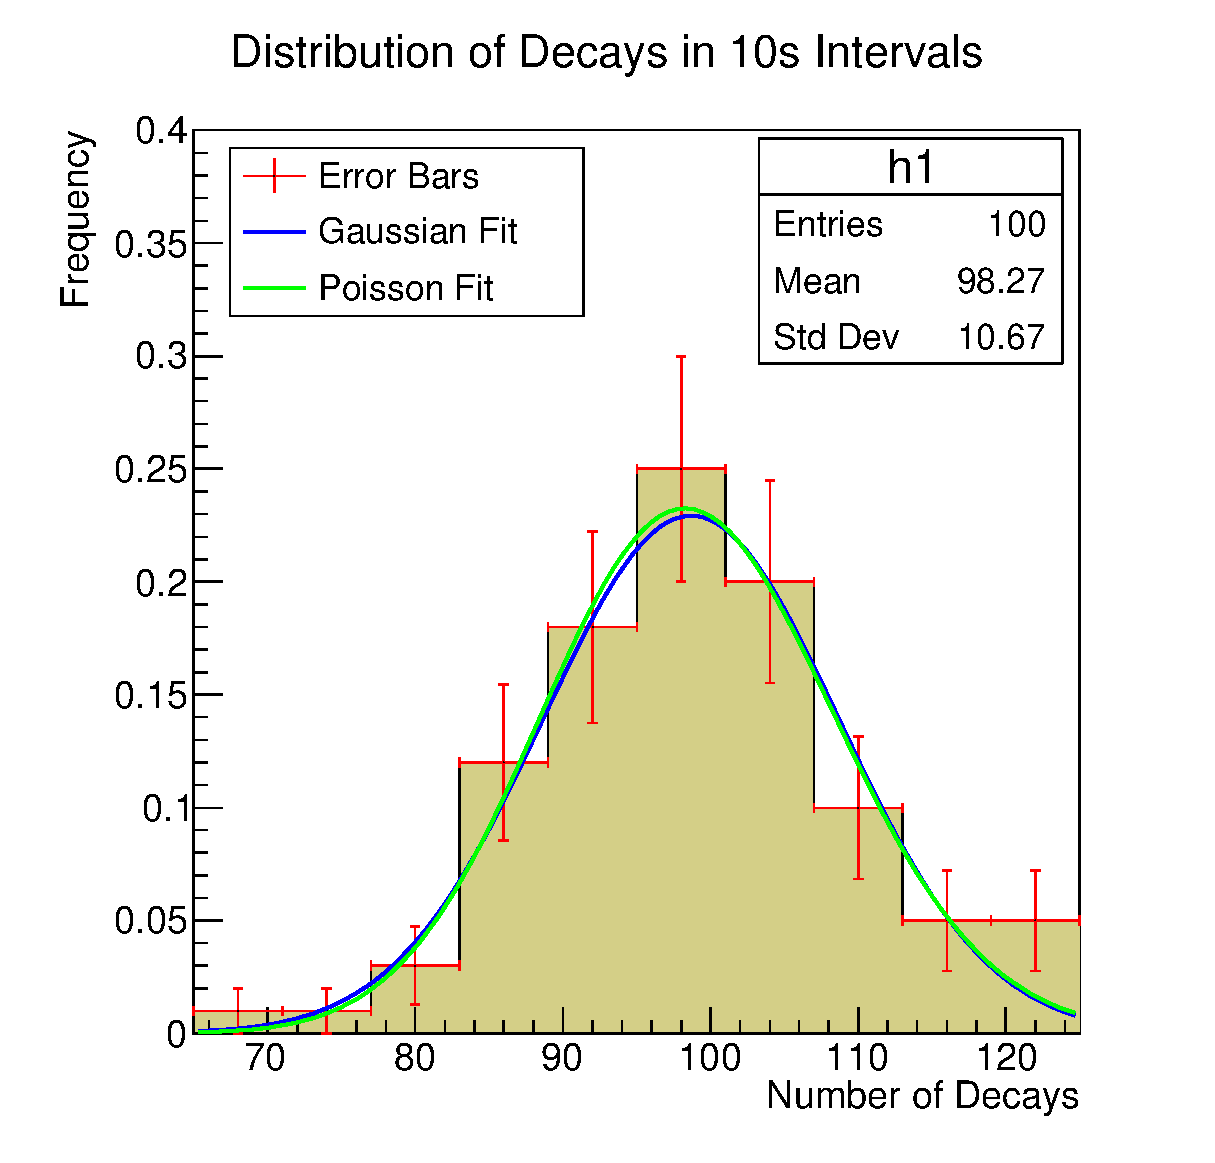
\includegraphics[width=\columnwidth]{graphics/10s.eps}
  \caption{Distribution of decays in 10s intervals. Total entries, mean and standard deviation is given.}
   \label{fig:10s}
\end{figure}


\begin{table}[H]
\caption{\label{tab:10sg}%
Calculations for gaussian fit applied to distribution of decays in 10s intervals. Chi square $\chi^2$, degree of freedom $\nu$, chi square per degree of freedom $\chi_\nu^2$, mean $\mu$ with error $\sigma_\mu$, standart deviation $\sigma$ with error $\sigma_\sigma$ and normalization constant $c$ with error $\sigma_c$ is given.}
\begin{ruledtabular}
\begin{tabular}{ccccccccc}
        \textrm{$\chi^2$}&
        \textrm{$\nu$}&
        \textrm{$\chi^2_v$}&
        \textrm{$\mu$} &
        \textrm{$\sigma_\mu$} &
        \textrm{$\sigma$}  &
        \textrm{$\sigma_\sigma$} &
        \textrm{$c$}  &
        \textrm{$c_\sigma$} \\ 
\colrule 
        4.280 & 7 & 0.611 & 98.67 & 1.10 & 10.03 & 0.97 & 5.77 & 0.59 
\end{tabular}  
\end{ruledtabular}
\end{table}

\begin{table}[H]
\caption{\label{tab:10ps}%
Calculations for poisson fit applied to distribution of decays in 10s intervals. Chi square $\chi^2$, degree of freedom $\nu$, chi square per degree of freedom $\chi_\nu^2$, mean $\mu$ with error $\sigma_\mu$ and normalization constant $c$ with error $\sigma_c$ is given.
}
\begin{ruledtabular}
\begin{tabular}{ccccccc}
        \textrm{$\chi^2$}&
        \textrm{$\nu$}&
        \textrm{$\chi^2_v$}&
        \textrm{$\mu$} &
        \textrm{$\sigma_\mu$} &
        \textrm{$c$}  &
        \textrm{$c_\sigma$} \\ 
\colrule 
        3.977 & 8 & 0.497 & 98.79 & 1.06 & 5.79 & 0.59 
\end{tabular}  
\end{ruledtabular}
\end{table}




\begin{figure}[H]
  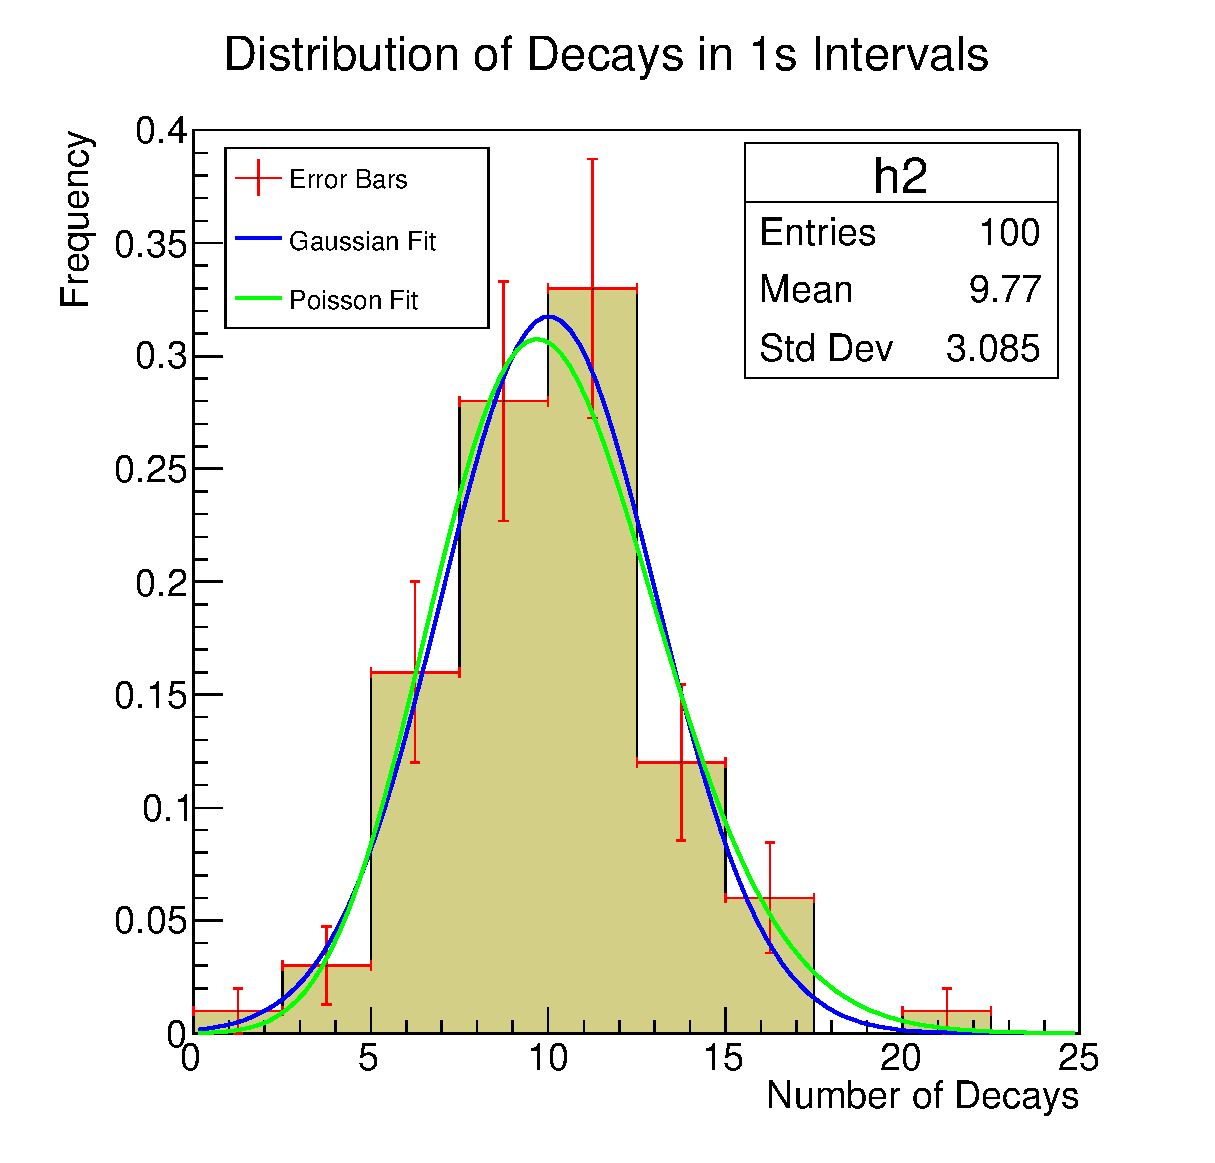
\includegraphics[width=\columnwidth]{graphics/1s.eps}
  \caption{Distribution of decays in 1s intervals. Total entries, mean and standard deviation is given.}
   \label{fig:1s}
\end{figure}


\begin{table}[H]
\caption{\label{tab:1sg}%
Calculations for gaussian fit applied to distribution of decays in 1s intervals. Chi square $\chi^2$, degree of freedom $\nu$, chi square per degree of freedom $\chi_\nu^2$, mean $\mu$ with error $\sigma_\mu$, standart deviation $\sigma$ with error $\sigma_\sigma$ and normalization constant $c$ with error $\sigma_c$ is given.
}
\begin{ruledtabular}
\begin{tabular}{ccccccccc}
        \textrm{$\chi^2$}&
        \textrm{$\nu$}&
        \textrm{$\chi^2_v$}&
        \textrm{$\mu$} &
        \textrm{$\sigma_\mu$} &
        \textrm{$\sigma$}  &
        \textrm{$\sigma_\sigma$}  &
        \textrm{$c$}  &
        \textrm{$c_\sigma$} \\ 
\colrule 
        3.432 & 5 & 0.686 & 10.02 & 0.33 & 3.05 & 0.29 & 2.43 & 0.25 
\end{tabular}  
\end{ruledtabular}
\end{table}

\begin{table}[H]
\caption{\label{tab:1ps}%
Calculations for poisson fit applied to distribution of decays in 1s intervals. Chi square $\chi^2$, degree of freedom $\nu$, chi square per degree of freedom $\chi_\nu^2$, mean $\mu$ with error $\sigma_\mu$ and normalization constant $c$ with error $\sigma_c$ is given.
}
\begin{ruledtabular}
\begin{tabular}{ccccccc}
        \textrm{$\chi^2$}&
        \textrm{$\nu$}&
        \textrm{$\chi^2_v$}&
        \textrm{$\mu$} &
        \textrm{$\sigma_\mu$} &
        \textrm{$c$}  &
        \textrm{$c_\sigma$} \\ 
\colrule 
        3.210 & 6 & 0.535 & 10.12 & 0.34 & 2.45 & 0.25
\end{tabular}  
\end{ruledtabular}
\end{table}


\subsubsection{Second Part}
This part, in order to show our time dependent poisson distribution is coherent, we binned the times passed between successive decays measured with analog chart recorder. Later, time dependent poisson fits \eqref{eq:time} applied to histograms.
\setcounter{secnumdepth}{4}

$n=0$ case, we get:
\begin{align}
        P(1,t) = \alpha e^{-\alpha t} \label{eq:n0}
\end{align}


\begin{figure}[H]
  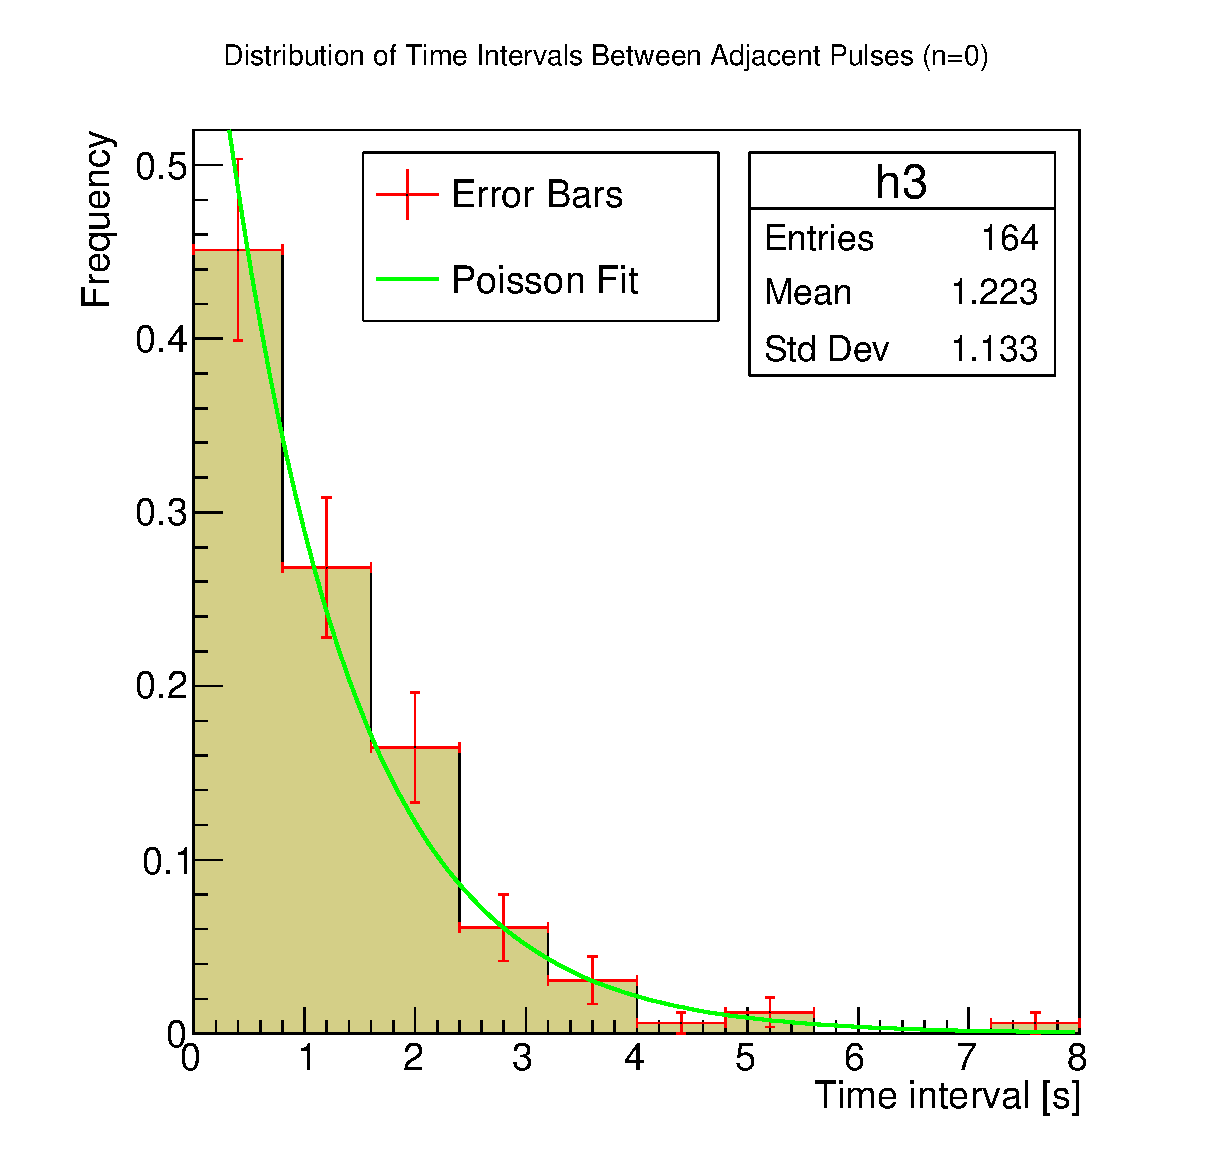
\includegraphics[width=\columnwidth]{graphics/p2_1.eps}
        \caption{Distribution of time intervals between adjacent pulses (n=0). Total entries, mean and standard deviation is given.}
   \label{fig:p2_1}
\end{figure}


\begin{table}[H]
\caption{\label{tab:1ps}%
        Calculations for time dependent poisson fit \eqref{eq:n0} applied to distribution of time intervals between adjacent pulses. Chi square $\chi^2$, degree of freedom $\nu$, chi square per degree of freedom $\chi_\nu^2$, average counts per unit time $\alpha$ with error $\sigma_\alpha$ and normalization constant $c$ with error $\sigma_c$ is given.
}
\begin{ruledtabular}
\begin{tabular}{ccccccc}
        \textrm{$\chi^2$}&
        \textrm{$\nu$}&
        \textrm{$\chi^2_v$}&
        \textrm{$\alpha$} &
        \textrm{$\sigma_\alpha$} &
        \textrm{$c$}  &
        \textrm{$c_\sigma$} \\ 
\colrule 
        5.904 & 6 & 0.984 & 0.87 & 0.07 & 0.79 & 0.06  
\end{tabular}  
\end{ruledtabular}
\end{table}


$n=1$ case, we get:
\begin{align}
        P(2,t) =  \alpha^2 t  e^{-\alpha t} \label{eq:n1}
\end{align}

To get the distribution, we added successive pairs of time intervals.


\begin{figure}[H]
  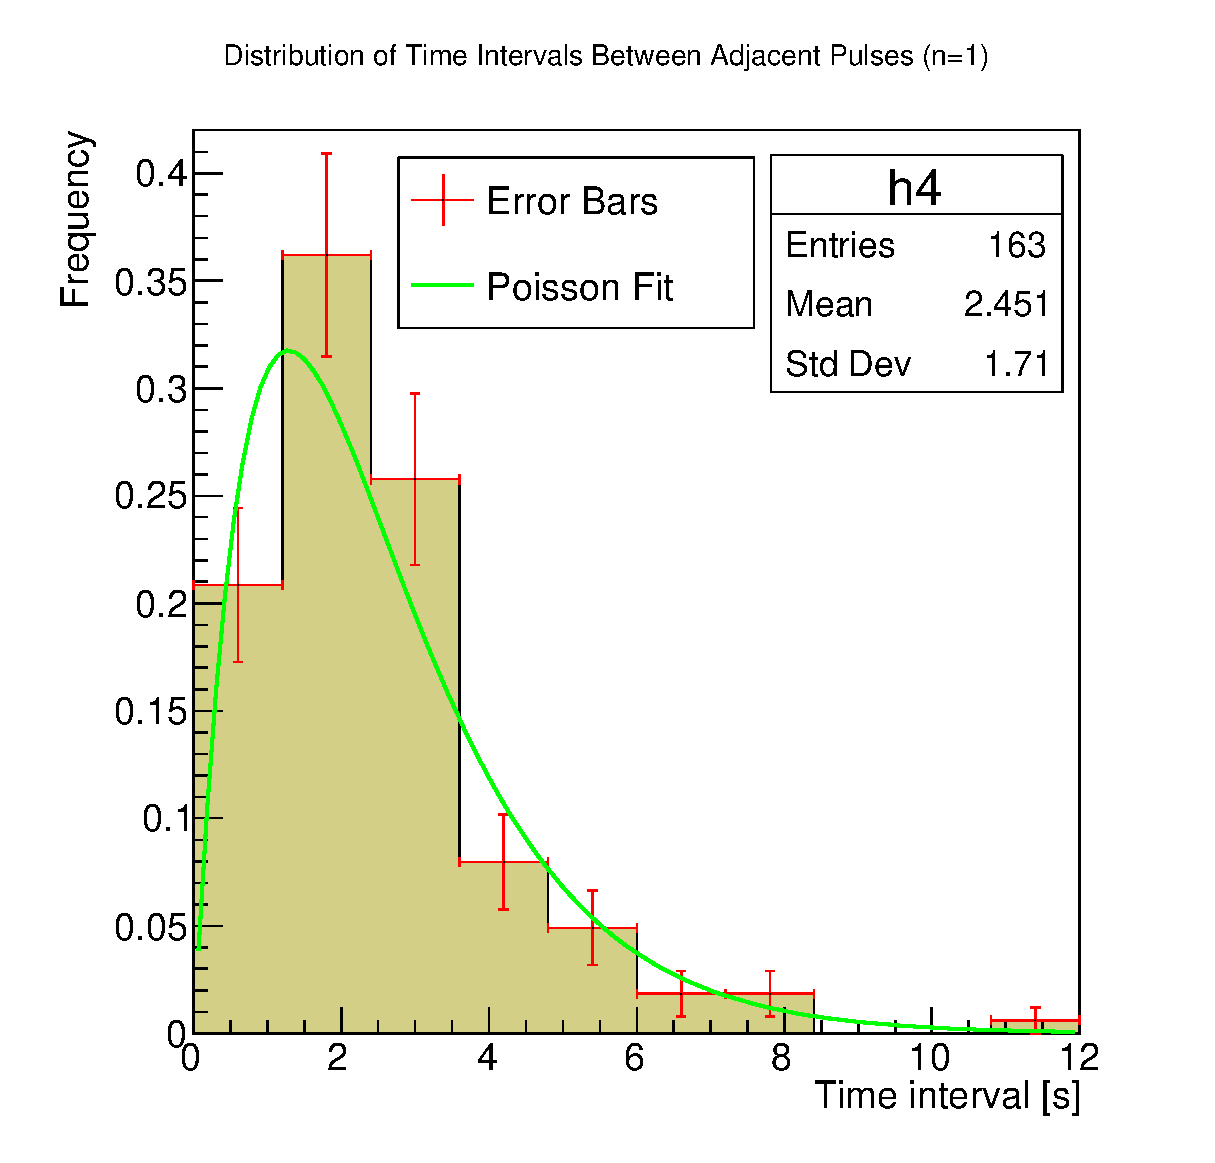
\includegraphics[width=\columnwidth]{graphics/p2_2.eps}
        \caption{Distribution of time intervals between adjacent pulses (n=1). Total entries, mean and standard deviation is given.}
   \label{fig:p2_2}
\end{figure}


\begin{table}[H]
\caption{\label{tab:2ps}%
        Calculations for time dependent poisson fit \eqref{eq:n1} applied to distribution of time intervals between adjacent pulses. Chi square $\chi^2$, degree of freedom $\nu$, chi square per degree of freedom $\chi_\nu^2$, average counts per unit time $\alpha$ with error $\sigma_\alpha$ and normalization constant $c$ with error $\sigma_c$ is given.
}
\begin{ruledtabular}
\begin{tabular}{ccccccc}
        \textrm{$\chi^2$}&
        \textrm{$\nu$}&
        \textrm{$\chi^2_v$}&
        \textrm{$\alpha$} &
        \textrm{$\sigma_\alpha$} &
        \textrm{$c$}  &
        \textrm{$c_\sigma$} \\ 
\colrule 
        9.036 & 6 & 1.50 & 0.78 & 0.04 & 1.11 & 0.09 
\end{tabular}  
\end{ruledtabular}
\end{table}




\section{Conclusion}
If we list our $\chi^2_v$ findings from the first part, we get:


\begin{table}[H]

\begin{ruledtabular}
\begin{tabular}{ccc}
        \textrm{Time interval $[s]$}&
        \textrm{Distribution}&
        \textrm{$\chi^2_v$} \\
\colrule 
        1 & Gaussian & 0.686 \\
        1 & Poisson  & 0.535 \\
        \hline 
        10 & Gaussian & 0.611 \\
        10 & Poisson  & 0.497 \\
\end{tabular}  
\end{ruledtabular}
\end{table}

Since our poisson fits have smaller $\chi^2_v$ values than gaussian ones, in radioactive decay using poisson distribution instead of gaussian distribution makes sense. The main reason of this result is all of our measurements are counting measurements which they are not continuous but discrete. 


If we look at second part we see acceptable $\chi^2_v$ values for time-dependent poisson distribution as well:


\begin{table}[H]
\begin{ruledtabular}
\begin{tabular}{@{\hspace{5em}} c c @{\hspace{5em}}}
        \textrm{n}&
        \textrm{$\chi^2_v$} \\
\colrule 
        0 & 0.984 \\
        1 & 1.500 \\
\end{tabular}  
\end{ruledtabular}
\end{table}
which again indicates that modelling radioactive decay with the poisson distribution is suitable. 

\subsection{Possible Error Sources}
Since, we did not physically conduct this experiment, it is difficult to say what went wrong. However, using different gamma-ray sources and taking more data can give more reliable results.







\newpage
\appendix
\section{Measurements}
All measurements are in this repository : \url{https://github.com/tanaytekin/phys442_poissonstatistics} 
\section{Mathematical Concepts}

\subsection{Chi-squared Test}
$\chi^2$ can be defined as:
\begin{align}
  \chi^2 = \sum \frac{(y_i -y(x_i))^2}{\sigma^2_i}
\end{align}
$\chi^2$ per degrees of freedom:
\begin{align}
  \chi^2_\nu = \frac{1}{\nu} \sum \frac{(y_i -y(x_i))^2}{\sigma^2_i}
\end{align}
where $\nu$ is the number of degrees of freedom; the number of data points minus the number of parameters: $N-m$.

\subsection{Least Squares Method}

Let's define line for fitting as $y_i = a_0 + a_1x_i$
Parameters are
\begin{align}
  a_0 &= \frac{1}{D}\left(\sum_{k}^{N}\frac{x^2_k}{\sigma^2_k} \sum_{k}^{N}\frac{y_k}{\sigma^2_k} - \sum_{k}^{N}\frac{x_k}{\sigma^2_k} \sum_{k}^{N}\frac{x_k y_k}{\sigma^2_k}\right) \\
    a_1 &= \frac{1}{D}\left(\sum_{k}^{N}\frac{1}{\sigma^2_k} \sum_{k}^{N}\frac{x_k y_k}{\sigma^2_k} - \sum_{k}^{N}\frac{x_k}{\sigma^2_k} \sum_{k}^{N}\frac{y_k}{\sigma^2_k}\right) \\
    D &= \sum_{k}^{N}\frac{1}{\sigma^2_k} \sum_{k}^{N}\frac{x^2_k}{\sigma^2_k} - \left(\sum_{k}^{N}\frac{x_k}{\sigma^2_k}\right)^2
\end{align}
Uncertainties of Parameters are:
\begin{align}
\sigma^2_{a_0} = \frac{1}{D} \sum_{k}^{N}\frac{x^2_j}{\sigma^2_j} \\
\sigma^2_{a_1} = \frac{1}{D} \sum_{k}^{N}\frac{1}{\sigma^2_j}
\end{align}

\subsection{Error Propagation}
\begin{align}
  \sigma^2_y = \sum_i^m \left(\frac{\partial f}{\partial x_i}\right)^2 \sigma^2_i \label{eq:err}
\end{align}

\subsection{Total Uncertainty}
\begin{align}
  \sigma^2 = \sigma_{systematic}^2 + \sigma_{instrumental}^2 + \sigma_{statistical}^2 \label{eq:unc}
\end{align}

\subsection{Weighted Mean and Standart Deviation} 
Mean:
\begin{align}
\mu = \frac{\sum\limits_i^N x_i / \sigma_i^2}{\sum\limits_i^N 1/\sigma_i^2} \label{eq:mean}
\end{align}
Standard Deviation:
\begin{align}
  \sigma^2 \simeq \frac{1}{\sum\limits_i^N 1/\sigma_i^2}  \label{eq:meanstd}
\end{align}


\newpage
\nocite{*}
\bibliography{report}

\end{document}
